\chapter{Experiments} % Main chapter title

\label{Chapter5} % For referencing the chapter elsewhere, use \ref{Chapter5} 

\lhead{Chapter 5. \emph{Experiments}} % This is for the header on each page - perhaps a shortened title

%----------------------------------------------------------------------------------------

In this chapter we will be discussing about two systems implemented to use \textit{sentiment analysis} in \textit{information retrieval}.
Also, \textit{LDA} was evaluated to test the accuracy of unsupervised approaches in general.

\begin{enumerate}
 \item Indexing followed by Sentiment Analysis
 \item Encoding sentiment in the Index
\end{enumerate}

As can be seen by the brief description, the first one uses a staged approach and the second one is a one-stage process but involves
some heavy preprocessing to predict the sentiment of the \textit{text}. These approaches are very simple and aren't novel.
These systems have merely been discussed to show the novelty of some future work. \textit{Lucene} \citep*{apachelucene} was used for indexing
in both these systems.

\section{Indexing followed by Sentiment Analysis}

\subsection{Architecture}

\begin{enumerate}
 \item Lucene
  \par It has a variety of features to perform indexing from basic to very advanced. 
 \item Query Processor
  \par This is also a part of of lucene. The objective content of the query is processed by this component
 \item Sentiment Analyzer
  \par Sentiwordnet \citep*{sentiwordnet} was used to calculate the score of each word. The sentiment for a sentence was a sum of sentiment scores
  for each word. Sentiment of the whole document was a sum of sentiments for all the sentences. 
\end{enumerate}

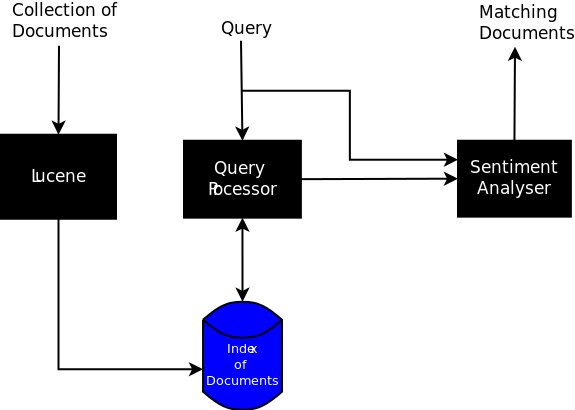
\includegraphics[width=\textwidth]{IndexingFollowedBySentimentAnalysis}
\begin{center}
 Figure 5.1 Indexing Followed by Sentiment Analysis
\end{center}

\section{Encoding sentiment in the Index}

\subsection{Architecture}

\begin{enumerate}
 \item Lucene + Sentiment Analyzer
  \par It has a variety of features to perform indexing from basic to very advanced. In this case, sentiment analysis was combined with
  indexing. One more field, \textit{sentiment} was added to the index. This value was inferred using the sentiment analyzer. 
 \item Query Processor
  \par In this case, both the subjective and objective content of the query was processed. The documents were fetched based on the objective
  content of the query. Then, depending on the value of the \textit{sentiment} field, these fetched documents were filtered and presented
  to the user.
\end{enumerate}

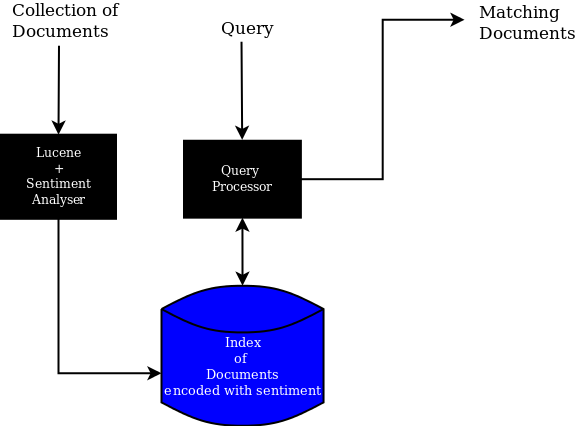
\includegraphics[width=\textwidth]{SentimentEncodedInIndex}
\begin{center}
 Figure 5.2 Encoding Sentiment in Index
\end{center}

Both these systems can be very useful. But as we can see the first one incurs lot of processing overhead and the second one has lot of 
preprocessing overhead. Also, both follow a procedural approach. A more novel approach will be two combine sentiment and topic to create 
a model which we can fit to our training data and then infer the resemblance of a new document to existing ones.

\section{Evaluation of LDA}

Evaluation of topic models has been discussed at length in \citep*{wallach2009evaluation}. A natural evaluation metric discussed in 
\citep*{wallach2009evaluation} is finding out the probability of a held-out document given a trained model. Topic modeling is a useful
tool for analyzing unstructured text collections. Evaluation of topic models is difficult due to their unsupervised nature. For some 
applications, there might be extrinsic tasks such as information retrieval for which performance can be evaluated. There is a need for 
a universal method that measures generalization capability of a topic model in a way that is accurate, computationally efficient and
independent of a specific application. \textit{LDA} can be evaluated by 1) Information retrieval accuracy or 2) by estimating the probability
of unseen held-out documents given some training documents. We propose a new evaluation method as follows.

\subsection*{Evaluation method}

\begin{enumerate}
 \item Download documents.
 \item Tag every document with a topic to get a tagged corpus
 \item Held-out some documents for testing before training the model
 \item Train the topic model using the untagged corpus (obtained after removing the tags)
 \item Now, use the trained model to infer topic distribution for the testing documents
 \item Check whether the topic having highest proportion matches the tag of the document
\end{enumerate}

5-fold cross validation was used in this case. 1273 documents were downloaded from DMOZ \citep*{dmoz}. Computers, films, real estate, cooking and
sports were the 5 topics chosen. The implementation in Mallet was used to conduct the experiment.

\begin{center}
\begin{tabular}{ |c|c| }
  \hline
  Topic & No. of files \\ \hline
  Computers & 164 \\ \hline
  Sports & 213 \\ \hline
  Cooking & 251 \\ \hline
  Real Estate & 261 \\ \hline
  Films & 384 \\ \hline
\end{tabular}
\end{center}
\begin{center}
 Table 5.1 Number of files per topic
\end{center}

\begin{center}
\begin{tabular}{ |c|c| }
  \hline
  Average accuracy & 20.867 \\ \hline
\end{tabular}
\end{center}
\begin{center}
 Table 5.2 Average Accuracy 
\end{center}

\subsection*{Discussion}

\par
The average accuracy after 5-fold cross-validation on this corpus was 20.867, which is very low. The reason for this is the short-length
of the documents used. \textit{LDA} works on the principle of co-occurrence. If we look at \eref{eqn:fullconditionalfinal}, there is a
factor for words and another for documents. Probabilities are higher for assignments that "don't break document boundaries", that is, words 
appearing in the same document have a slightly higher odds of ending up in the same topic. The same holds for document assignments, they to 
a degree follow "word boundaries". These effects mix up and spread over clusters of documents and words, eventually. Due to the short length 
of the documents, words from the same topic may not always co-occur. Also, there is chance of them co-occurring with words from other topics 
also which results in bad clustering. Some words belong to more than one topic due to this. Due to this, the clustering of documents as whole 
in this case is not good. 

\par
Also, the evaluation method used is very strict. If it is a bit lenient, the accuracy can be increased. A new method
called weighted evaluation can be used in this case.

\subsection*{Weighted Evaluation}

Weighted evaluation is based on the fact that we get a topic distribution for each testing document. This topic distribution is arranged
in descending order of topic proportions. The idea is to assign weights according to the rank given to the original tag of the document. 

\subsection*{Weighted Evaluation Algorithm}

\begin{alltt}
matches=0, counts=0
For each document
  Find topic distribution
  Switch(tag):
    case(topic1): matches += 1
    case(topic2): matches += 0.8
    case(topic3): matches += 0.6
    case(topic4): matches += 0.4
    case(topic5): matches += 0.2
    counts++
Accuracy = matches/counts
\end{alltt}

\subsection*{Results}

\begin{center}
\begin{tabular}{ |c|c|c|c| }
  \hline
  Fold & Matches & Counts & Accuracy (in percentage) \\ \hline
  Fold 1 & 156 & 255 & 61.4 \\ \hline
  Fold 2 & 156 & 255 & 61.4 \\ \hline
  Fold 3 & 170 & 255 & 66.9 \\ \hline
  Fold 4 & 152 & 255 & 59.6 \\ \hline
  Fold 5 & 161 & 253 & 63.9 \\ \hline
\end{tabular}
\end{center}
\begin{center}
 Table 5.3 Accuracy for each testing fold 
\end{center}

\begin{center}
\begin{tabular}{ |c|c| }
  \hline
  Average accuracy & 62.6 \\ \hline
\end{tabular}
\end{center}
\begin{center}
 Table 5.4 Weighted Evaluation Average Accuracy 
\end{center}

\subsection*{Discussion}

\par
As we can see the accuracy has increased after we used weighted evaluation. This kind of evaluation needs to be used in many systems including
transliteration where the most probable word needs to be predicted. The rank of the actual word may be further down. This doesn't mean that the
system is giving wrong output. Therefore, a more lenient approach would be better in this case. 

\par
The accuracy has increased but still is unsatisfactory. 62 \% accuracy in this case implies that given a document, there is 62 \%
chance that the main topic of the document will be ranked in top 5. As we have used only 5 topics, this result is not that significant. Using
more number of topics will lead to better insights. 

\par 
If we consider the clustering to be effective only till the third rank, we get accuracies as shown in the table.

\begin{center}
\begin{tabular}{ |c|c|c|c| }
  \hline
  Fold & Matches & Counts & Accuracy (in percentage) \\ \hline
  Fold 1 & 156 & 255 & 50.9 \\ \hline
  Fold 2 & 156 & 255 & 50.1 \\ \hline
  Fold 3 & 170 & 255 & 57.4 \\ \hline
  Fold 4 & 152 & 255 & 46.7 \\ \hline
  Fold 5 & 161 & 253 & 53.5 \\ \hline
\end{tabular}
\end{center}
\begin{center}
 Table 5.5 Accuracy for each testing fold (Till 3rd rank)
\end{center}

\begin{center}
\begin{tabular}{ |c|c| }
  \hline
  Average accuracy & 51.7 \\ \hline
\end{tabular}
\end{center}
\begin{center}
 Table 5.6 Average Accuracy (Till 3rd rank)
\end{center}

\par 

This means that given a document, there is 51.7 \% chance that the main topic of the document will be ranked in top 3. It is known
that \textit{LDA} performs better with more number of topics. So, increasing the number of topics while performing the evaluation can 
lead to more better results. 

A list of high probability words for each topic was prepared which is given in the following table. 

\begin{center}
\begin{tabular}{ |c|c|c|c|c| }
  \hline \hline
  Computer & Films & Cooking & Real Estate & Sports \\ \hline \hline
  site & film &	recipes & services & reviews \\ \hline
  software & information & recipe & real & news \\ \hline
  free & offers & including & company &	interviews\\ \hline
  systems & production & collection & estate & information \\ \hline
  programming & courses & tips & includes & features \\ \hline
  research & links & source & commercial & current \\ \hline
  resources & videos & production & based & tennis \\ \hline
  code & television & baking & development & running \\ \hline
  information &	cinema & breakfast & title & tournament \\ \hline
\end{tabular}
\end{center}
\begin{center}
 Table 5.7 High probability words in each topic 
\end{center}

As we can see, the high probability words in each topic are good but due to the short length, results were not that good. 

\section*{Summary}
In this chapter, we discussed two systems that implement sentiment analysis in information retrieval using a procedural approach. Also,
the pros and cons of these systems have been discussed. Also, the evaluation of \textit{LDA} has been discussed.

In the next chapter, we conclude and comment on some future work.

\clearpage